\documentclass[14pt,a4paper]{scrartcl}
\usepackage{cmap}
\usepackage[utf8]{inputenc}
\usepackage[T1,T2A]{fontenc}
\usepackage[english,russian]{babel}
\usepackage{relsize}
\usepackage{graphicx}
\usepackage{subfigure}
\usepackage{mathtools}
\usepackage{amssymb}
\usepackage{float}
\usepackage{sidecap}
\usepackage{wrapfig}
\usepackage{caption}
\usepackage[table,xcdraw]{xcolor}
\usepackage{minted}
\usepackage{physics}
\DeclareMathOperator\atanh{arctanh}
\begin{document}
	\begin{titlepage}
	\begin{center}
		\large
		МИНИСТЕРСТВО ОБРАЗОВАНИЯ И НАУКИ\\ РОССИЙСКОЙ ФЕДЕРАЦИИ
		
		\vspace{0.5cm}
		
		МГТУ им Н.Э.Баумана
		\vspace{0.25cm}
		
		Факультет ФН
		
		Кафедра вычислительной математики и математической физики
		\vfill
		
		
		Соколов Арсений Андреевич\\
		\vfill
		
		
		{\LARGE Домашнее задание №8 по математической статистике\\[2mm]
		}
		\bigskip
		
		3 курс, группа ФН11-53Б\\
		Вариант 9
	\end{center}
	\vfill
	
	\newlength{\ML}
	\settowidth{\ML}{«\underline{\hspace{0.7cm}}» \underline{\hspace{2cm}}}
	\hfill\begin{minipage}{0.4\textwidth}
		Преподаватель\\
		\underline{\hspace{3cm}} Т.\,В.~Облакова\\
		«\underline{\hspace{0.7cm}}» \underline{\hspace{1.71cm}} 2019 г.
	\end{minipage}%
	\bigskip
	
	
	\vfill
	
	\begin{center}
		Москва, 2019 г.
	\end{center}
\end{titlepage}

\section*{Задание 1}


Смоделировать выборку $(X_k, Y_k)$ из двумерного гауссовского распределения объёма $n=140$ с данными параметрами $\vec{\mu} = \begin{pmatrix} a \\ b \end{pmatrix} = \begin{pmatrix} 1 \\ -3 \end{pmatrix}$ и $\Sigma = \begin{pmatrix}
\sigma_{11} & \sigma_{12}\\
\sigma_{21} & \sigma_{22}
\end{pmatrix} =  \begin{pmatrix}
1 & -1\\
-1 & 2
\end{pmatrix}$. Построить двумерную гистограмму и диаграмму рассеяния полученной выборки.\\
\textbf{Решение.}\\

Пусть $(\xi, \eta)$ -- - гауссовский вектор с параметрами $\vec{\mu} = \begin{pmatrix} a \\ b \end{pmatrix}$ и $\Sigma = \begin{pmatrix}
	\sigma_{11} & \sigma_{12}\\
	\sigma_{21} & \sigma_{22}
\end{pmatrix}$\\
Пусть 
\begin{equation*}
	\eta = b + \frac{\sigma_{12}}{\sigma_{11}}(\xi - a) + \varepsilon
\end{equation*}

Тогда $\varepsilon \sim N(0, \sqrt{\sigma_{22}(1-r^2)})$ и не зависит от $\xi$, $r = \frac{\sigma_{12}}{\sqrt{\sigma_{11}\sigma_{22}}}$.\\	

Воспользуемся этим фактом в моделировании нашей выборки:

\begin{equation*}
r = \frac{\sigma_{12}}{\sqrt{\sigma_{11}\sigma_{22}}} = \frac{-1}{\sqrt{1 \cdot 2}} = -0.7071068
\end{equation*}

\begin{equation*}
	X \sim N(a, \sqrt{\sigma_{11}}) \Leftrightarrow X \sim N(1,1)
\end{equation*}

\begin{equation*}
	\varepsilon \sim N(0, \sqrt{\sigma_{22}(1-r^2)}) \Leftrightarrow \varepsilon \sim N(0,1)
\end{equation*}

\begin{minted}{R}
> alpha <- 0.05
> n <- 140
> mu <- c(1,-3)
> Sigma <- matrix(c(1,-1,-1,2), byrow = T, ncol = 2)
> x <- rnorm(n,mu[1], sqrt(Sigma[1,1]))
> r <- Sigma[1,2] / sqrt(Sigma[1,1]*Sigma[2,2])
> r
[1] -0.7071068
> eps_k <- rnorm(n,mean = 0, sqrt(Sigma[2,2]*(1-r^2)))
> y <- mu[2] + Sigma[1,2]/Sigma[1,1] * (x-mu[1]) + eps_k
> df <- matrix(c(x,y,eps_k), ncol = 3)
\end{minted}


Получаемая выборка имеет вид:
\clearpage
\begin{table}[ht]
	\centering
	\begin{tabular}{|c||c||c||c|}
		\hline
		& x & y & $\varepsilon$ \\ 
		\hline
		1 & 0.15914 & -2.95514 & -0.79599 \\ 
		\hline
		2 & 2.38436 & -4.41371 & -0.02935 \\ 
		\hline
		3 & -0.25549 & 0.43573 & 2.18024 \\ 
		\hline
		4 & 1.07014 & -2.11272 & 0.95742 \\ 
		\hline
		5 & 2.71144 & -5.01649 & -0.30505 \\ 
		\hline
		6 & 0.39709 & -2.81550 & -0.41840 \\ 
		\hline
		7 & 0.52783 & -2.42788 & 0.09995 \\ 
		\hline
		8 & 0.36463 & -2.59444 & -0.22981 \\ 
		\hline
		9 & 0.71423 & -4.12944 & -1.41521 \\ 
		\hline
		10 & 1.13811 & -3.53071 & -0.39260 \\ 
		\hline
		11 & 2.22763 & -3.28154 & 0.94609 \\ 
		\hline
		12 & 0.19822 & -1.44645 & 0.75177 \\ 
		\hline
		13 & -0.08039 & -2.43698 & -0.51738 \\ 
		\hline
		14 & 0.84247 & -2.03413 & 0.80834 \\ 
		\hline
		15 & -0.07176 & -2.54278 & -0.61454 \\ 
		\hline
		16 & 0.86101 & -1.62275 & 1.23826 \\ 
		\hline
		17 & 0.40269 & -2.74078 & -0.33810 \\ 
		\hline
		18 & -1.18397 & 0.38033 & 1.19637 \\ 
		\hline
		19 & 1.24082 & -3.68414 & -0.44332 \\ 
		\hline
		20 & 0.74064 & -2.55453 & 0.18611 \\ 
		\hline
		21 & 1.90051 & -6.52186 & -2.62134 \\ 
		\hline
		22 & 1.94187 & -1.69561 & 2.24625 \\ 
		\hline
		23 & 2.46796 & -4.37453 & 0.09343 \\ 
		\hline
		24 & 1.70676 & -2.07948 & 1.62728 \\ 
		\hline
		25 & 1.81901 & -4.32993 & -0.51092 \\ 
		\hline
		26 & 0.70652 & -3.36590 & -0.65938 \\ 
		\hline
		27 & 2.41859 & -4.45878 & -0.04019 \\ 
		\hline
		28 & 2.49877 & -4.61747 & -0.11869 \\ 
		\hline
		29 & 0.34292 & -2.36257 & -0.01966 \\ 
		\hline
		30 & 0.14720 & -2.63288 & -0.48568 \\ 
		\hline
		31 & 1.31592 & -4.75606 & -1.44015 \\ 
		\hline
		32 & 2.10969 & -3.96593 & 0.14377 \\ 
		\hline
		33 & 3.21546 & -6.45005 & -1.23459 \\ 
		\hline
		34 & 2.21710 & -5.96960 & -1.75250 \\ 
		\hline
		35 & 2.47922 & -4.51472 & -0.03550 \\ 
		\hline
		36 & 1.95157 & -3.61954 & 0.33203 \\ 
		\hline
		37 & -0.00953 & -0.41818 & 1.57229 \\ 
		\hline
		38 & -1.00047 & -2.06900 & -1.06947 \\ 
		\hline
		39 & -0.76219 & -0.32153 & 0.91629 \\ 
		\hline
		40 & 0.85739 & -3.45238 & -0.59499 \\ 	
	\end{tabular}
\end{table}
\begin{table}[ht]
	\centering
	\begin{tabular}{|c||c||c||c|}
		41 & 2.55006 & -2.36841 & 2.18165 \\ 
	\hline
	42 & 0.19758 & -2.88135 & -0.68377 \\ 
	\hline
	43 & 0.92542 & -2.17536 & 0.75006 \\ 
	\hline
	44 & 2.89567 & -3.92129 & 0.97438 \\ 
	\hline
	45 & 0.54343 & -3.80790 & -1.26447 \\ 
	\hline
	46 & 1.56222 & -3.83964 & -0.27742 \\ 
	\hline
	47 & 0.11299 & -2.30239 & -0.18940 \\ 
	\hline
	48 & 0.53976 & -2.92378 & -0.38402 \\ 
	\hline
	49 & 0.27567 & -1.53508 & 0.74059 \\ 
	\hline
	50 & 0.93079 & -4.09913 & -1.16834 \\ 
	\hline
	51 & 2.46325 & -3.79571 & 0.66754 \\ 
	\hline
	52 & 1.18773 & -2.82149 & 0.36624 \\ 
	\hline
	53 & 2.02202 & -4.53697 & -0.51494 \\ 
	\hline
	54 & 0.40817 & -1.95760 & 0.45057 \\ 
	\hline
	55 & 0.88780 & -3.07552 & -0.18772 \\ 
	\hline
	56 & 0.07505 & -0.73598 & 1.33907 \\ 
	\hline
	57 & 1.75330 & -2.93709 & 0.81622 \\ 
	\hline
	58 & 0.88739 & -2.80519 & 0.08220 \\ 
	\hline
	59 & 0.93591 & -3.58677 & -0.65086 \\ 
	\hline
	60 & 1.23328 & -2.50687 & 0.72641 \\ 
	\hline
	61 & -0.13658 & -1.97710 & -0.11368 \\ 
	\hline
	62 & 1.85483 & -4.14993 & -0.29510 \\ 
	\hline
	63 & 0.42163 & -1.43246 & 0.98917 \\ 
	\hline
	64 & 1.49636 & -4.27149 & -0.77513 \\ 
	\hline
	65 & 0.23994 & -1.96404 & 0.27590 \\ 
	\hline
	66 & 0.65861 & -2.24783 & 0.41078 \\ 
	\hline
	67 & -1.10233 & -0.28649 & 0.61118 \\ 
	\hline
	68 & 0.69830 & -1.76173 & 0.93657 \\ 
	\hline
	69 & -0.27238 & -2.09516 & -0.36754 \\ 
	\hline
	70 & 0.72033 & -1.97996 & 0.74038 \\ 
	\hline
	71 & 0.79590 & -1.57737 & 1.21853 \\ 
	\hline
	72 & 0.77439 & -2.14525 & 0.62913 \\ 
	\hline
	73 & 1.34703 & -2.81928 & 0.52775 \\ 
	\hline
	74 & 1.03237 & -3.50462 & -0.47226 \\ 
	\hline
	75 & 1.41353 & -2.58982 & 0.82372 \\ 
	\hline
	76 & 0.84465 & -3.27244 & -0.42779 \\ 
	\hline
	77 & 1.97349 & -4.11613 & -0.14264 \\ 
	\hline
	78 & 1.12109 & -1.70231 & 1.41878 \\ 
	\hline
	79 & 1.18917 & -2.70204 & 0.48713 \\ 
	\hline
	80 & 0.43711 & -1.83367 & 0.60344 \\ 		
	\end{tabular}
\end{table}
\begin{table}[ht]
	\centering
	\begin{tabular}{|c||c||c||c|}
	81 & 1.49842 & -3.28758 & 0.21083 \\ 
	\hline
	82 & -0.74230 & -1.29100 & -0.03330 \\ 
	\hline
	83 & 1.97553 & -1.95033 & 2.02520 \\ 
	\hline
	84 & 0.97592 & -3.34670 & -0.37079 \\ 
	\hline
	85 & 1.67568 & -5.25392 & -1.57823 \\ 
	\hline
	86 & 0.28969 & -2.41126 & -0.12157 \\ 
	\hline
	87 & 3.38723 & -7.18391 & -1.79668 \\ 
	\hline
	88 & 0.52657 & -3.00216 & -0.47559 \\ 
	\hline
	89 & 0.92423 & -3.80833 & -0.88410 \\ 
	\hline
	90 & 0.47816 & -5.97622 & -3.49806 \\ 
	\hline
	91 & 1.92605 & -4.30803 & -0.38198 \\ 
	\hline
	92 & -0.06241 & -0.95990 & 0.97769 \\ 
	\hline
	93 & 1.55703 & -4.11507 & -0.55804 \\ 
	\hline
	94 & 1.90073 & -4.52719 & -0.62646 \\ 
	\hline
	95 & 1.98995 & -4.52040 & -0.53045 \\ 
	\hline
	96 & 1.38361 & -1.48599 & 1.89762 \\ 
	\hline
	97 & 0.65342 & -1.25788 & 1.39554 \\ 
	\hline
	98 & 0.45981 & -3.20584 & -0.74603 \\ 
	\hline
	99 & 0.81744 & -3.12302 & -0.30557 \\ 
	\hline
	100 & 0.94070 & -1.77102 & 1.16968 \\ 
	\hline
	101 & -0.99539 & -0.70023 & 0.30439 \\ 
	\hline
	102 & 2.13531 & -4.25281 & -0.11750 \\ 
	\hline
	103 & 1.67579 & -3.73588 & -0.06009 \\ 
	\hline
	104 & 1.20848 & -1.73754 & 1.47094 \\ 
	\hline
	105 & 0.94215 & -4.42030 & -1.47815 \\ 
	\hline
	106 & 1.89381 & -4.57742 & -0.68361 \\ 
	\hline
	107 & 0.77113 & -2.31059 & 0.46054 \\ 
	\hline
	108 & -0.96565 & -1.21585 & -0.18150 \\ 
	\hline
	109 & 0.24649 & -3.40531 & -1.15882 \\ 
	\hline
	110 & 2.28015 & -3.87113 & 0.40902 \\ 
	\hline
	111 & 0.04710 & -2.30530 & -0.25821 \\ 
	\hline
	112 & 2.62238 & -4.88928 & -0.26690 \\ 
	\hline
	113 & 3.60014 & -5.43599 & 0.16416 \\ 
	\hline
	114 & 1.13965 & -3.53311 & -0.39346 \\ 
	\hline
	115 & -0.35072 & -3.49302 & -1.84374 \\ 
	\hline
	116 & 1.79893 & -5.34122 & -1.54229 \\ 
	\hline
	117 & -0.55500 & -2.03124 & -0.58624 \\ 
	\hline
	118 & 1.46372 & -4.31586 & -0.85214 \\ 
	\hline
	119 & 1.05243 & -2.27411 & 0.77832 \\ 
	\hline
	120 & 0.79797 & -2.82829 & -0.03032 \\ 		
	\end{tabular}
\end{table}
	
\begin{table}[ht]
	\centering
	\begin{tabular}{|c||c||c||c|}
	\hline
	121 & 2.17086 & -5.62651 & -1.45566 \\ 
	\hline
	122 & 1.88484 & -3.79106 & 0.09378 \\ 
	\hline
	123 & -0.31789 & -0.69976 & 0.98235 \\ 
	\hline
	124 & -0.64325 & -1.95346 & -0.59671 \\ 
	\hline
	125 & 2.05925 & -3.98445 & 0.07480 \\ 
	\hline
	126 & 1.29008 & -1.09265 & 2.19743 \\ 
	\hline
	127 & 0.59997 & -1.80494 & 0.79502 \\ 
	\hline
	128 & 2.24310 & -4.78204 & -0.53894 \\ 
	\hline
	129 & -0.36641 & -3.23487 & -1.60128 \\ 
	\hline
	130 & -0.44141 & -2.28996 & -0.73137 \\ 
	\hline
	131 & 2.34855 & -4.70429 & -0.35574 \\ 
	\hline
	132 & -0.97853 & -2.00689 & -0.98541 \\ 
	\hline
	133 & -0.24095 & -2.49022 & -0.73117 \\ 
	\hline
	134 & 0.89596 & -1.43064 & 1.46532 \\ 
	\hline
	135 & 1.73297 & -1.87436 & 1.85862 \\ 
	\hline
	136 & 1.45568 & -3.45218 & 0.00350 \\ 
	\hline
	137 & 1.28808 & -4.63185 & -1.34378 \\ 
	\hline
	138 & -0.07369 & -1.77502 & 0.15129 \\ 
	\hline
	139 & 1.64874 & -3.35873 & 0.29001 \\ 
	\hline
	140 & 1.29916 & -3.42164 & -0.12248 \\ 
	\hline		
	\end{tabular}
\end{table}

\pagebreak
\clearpage
\begin{minted}{R}
> summary(df)
x                 y                eps           
Min.   :-1.1840   Min.   :-7.1839   Min.   :-3.498059  
1st Qu.: 0.3592   1st Qu.:-4.0131   1st Qu.:-0.565091  
Median : 0.9333   Median :-2.9026   Median :-0.115588  
Mean   : 1.0131   Mean   :-3.0172   Mean   :-0.004149  
3rd Qu.: 1.8039   3rd Qu.:-2.0002   3rd Qu.: 0.729901  
Max.   : 3.6001   Max.   : 0.4357   Max.   : 2.246255  
> var(df[,1]) # Дисперсия x
[1] 1.006593
> var(df[,2]) # Дисперсия y
[1] 1.996038
> var(df[,3]) # Дисперсия eps
[1] 0.9753832
\end{minted}

По полученной выборке построим двумерную гистограмму:
\begin{minted}{R}
> num_bins <- length(hist(df[,2], breaks = "Sturges", freq = T)$breaks)
> x_c <- cut(df[,1], num_bins)
> y_c <- cut(df[,2], num_bins)
> z <- table(x_c, y_c)
> library(plot3D)
> 
> main_perspective1 <- hist3D(x = seq(from = floor(min(df[,1])), 
+                                     ceiling(max(df[,1])), 
+                                     length.out = nrow(z)),
+                             y = seq(from = floor(min(df[,2])), 
+                                     ceiling(max(df[,2])), 
+                                     length.out = nrow(z)), 
+                             z=z, border="black", 
+                             ticktype = "detailed", lighting=T, 
+                             bty = "g", phi = 30, theta = 40, 
+                             lphi = 50)
> 
> main_perspective2 <- hist3D(x = seq(from = floor(min(df[,1])), 
+                                     ceiling(max(df[,1])), 
+                                     length.out = nrow(z)),
+                             y = seq(from = floor(min(df[,2])), 
+                                     ceiling(max(df[,2])), 
+                                     length.out = nrow(z)),
+                             z=z, border="black", 
+                             ticktype = "detailed", lighting=T, 
+                             bty = "g", phi = 30, theta = 80, 
+                             lphi = 50)
> 
> main_perspective3 <- hist3D(x = seq(from = floor(min(df[,1])), 
+                                     ceiling(max(df[,1])), 
+                                     length.out = nrow(z)),
+                             y = seq(from = floor(min(df[,2])), 
+                                     ceiling(max(df[,2])), 
+                                     length.out = nrow(z)),
+                             z=z, border="black", 
+                             ticktype = "detailed", lighting=T, 
+                             bty = "g", phi = 30, theta = 120, 
+                             lphi = 50)
> 
> main_perspective4 <- hist3D(x = seq(from = floor(min(df[,1])), 
+                                     ceiling(max(df[,1])), 
+                                     length.out = nrow(z)),
+                             y = seq(from = floor(min(df[,2])), 
+                                     ceiling(max(df[,2])), 
+                                     length.out = nrow(z)),
+                             z=z, border="black", 
+                             ticktype = "detailed", lighting=T, 
+                             bty = "g", phi = 30, theta = 160, 
+                             lphi = 50)
> plot(df)
\end{minted}

\begin{figure}[H]
	\begin{minipage}[h]{1\linewidth}
		\center{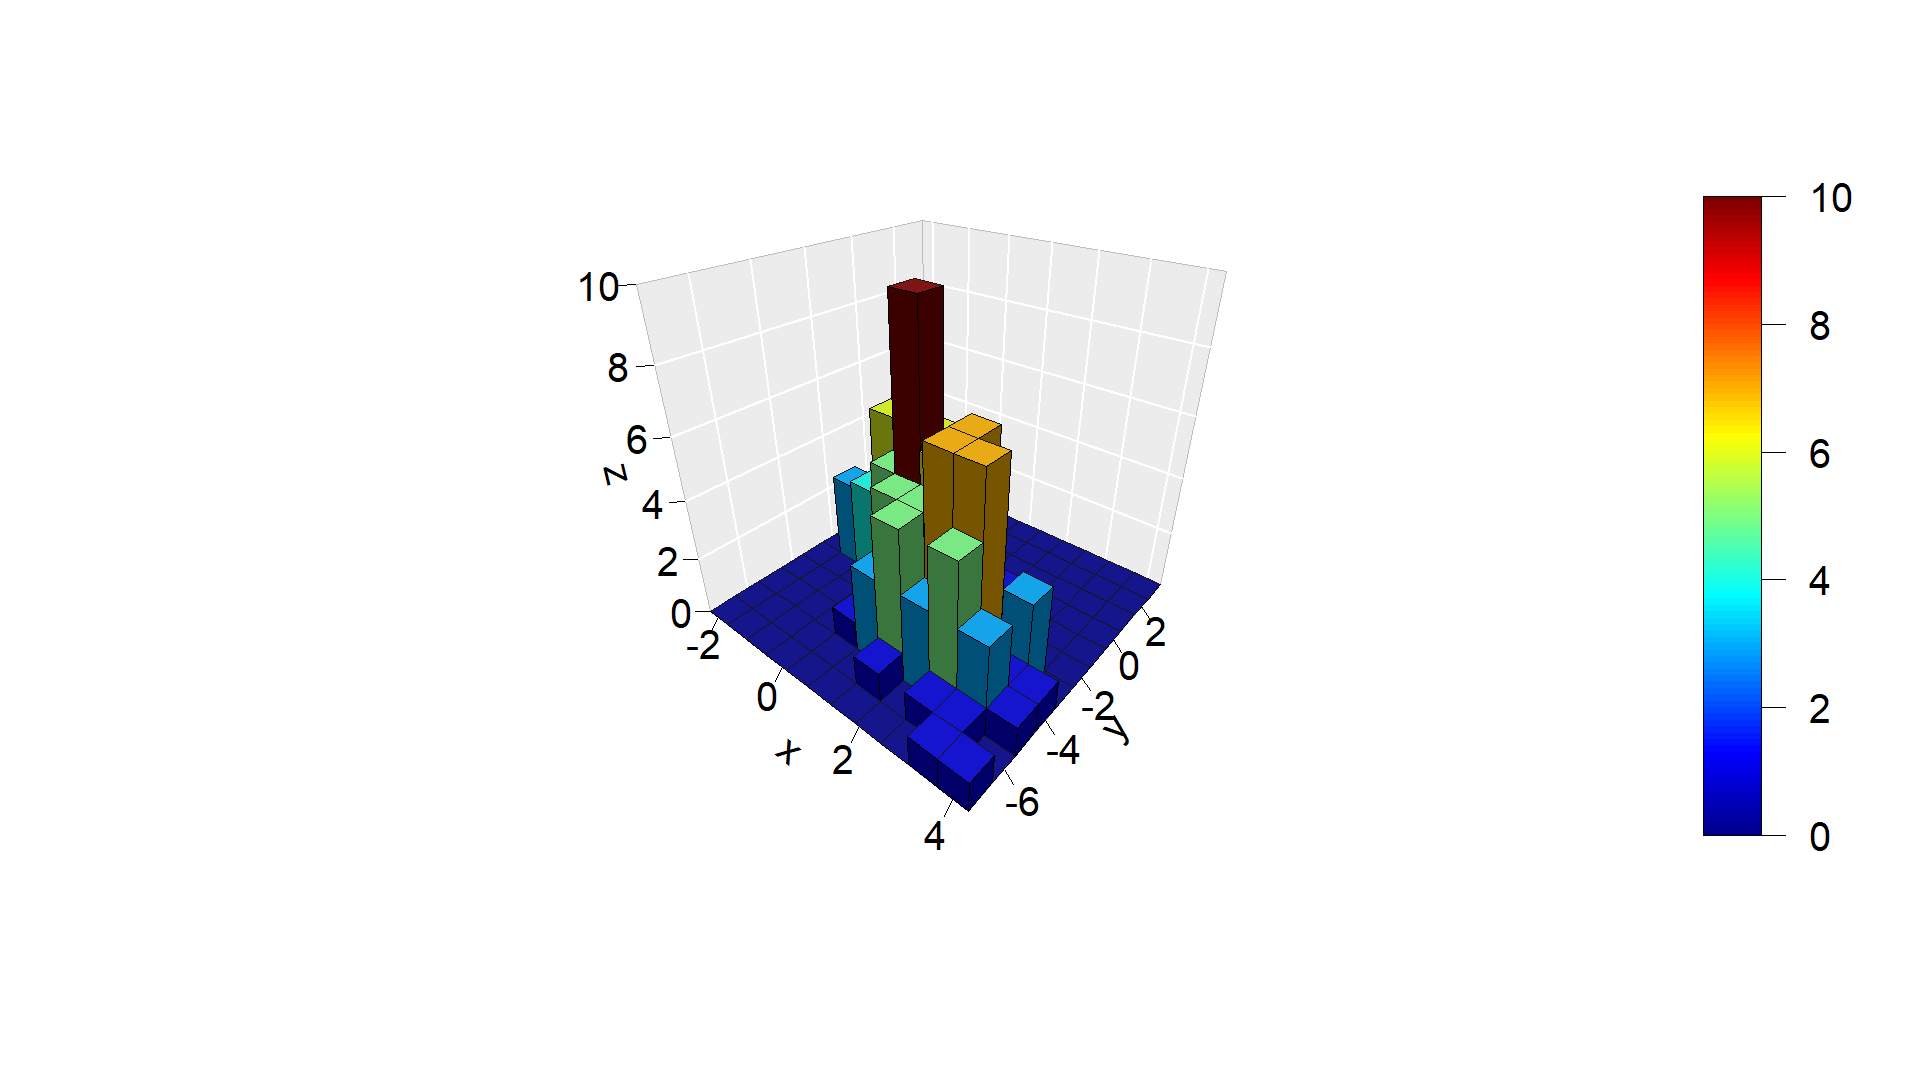
\includegraphics[width=1\linewidth]{../img/2d_1.png}}  \\
	\end{minipage}
	\hfill
	\begin{minipage}[h]{1\linewidth}
		\center{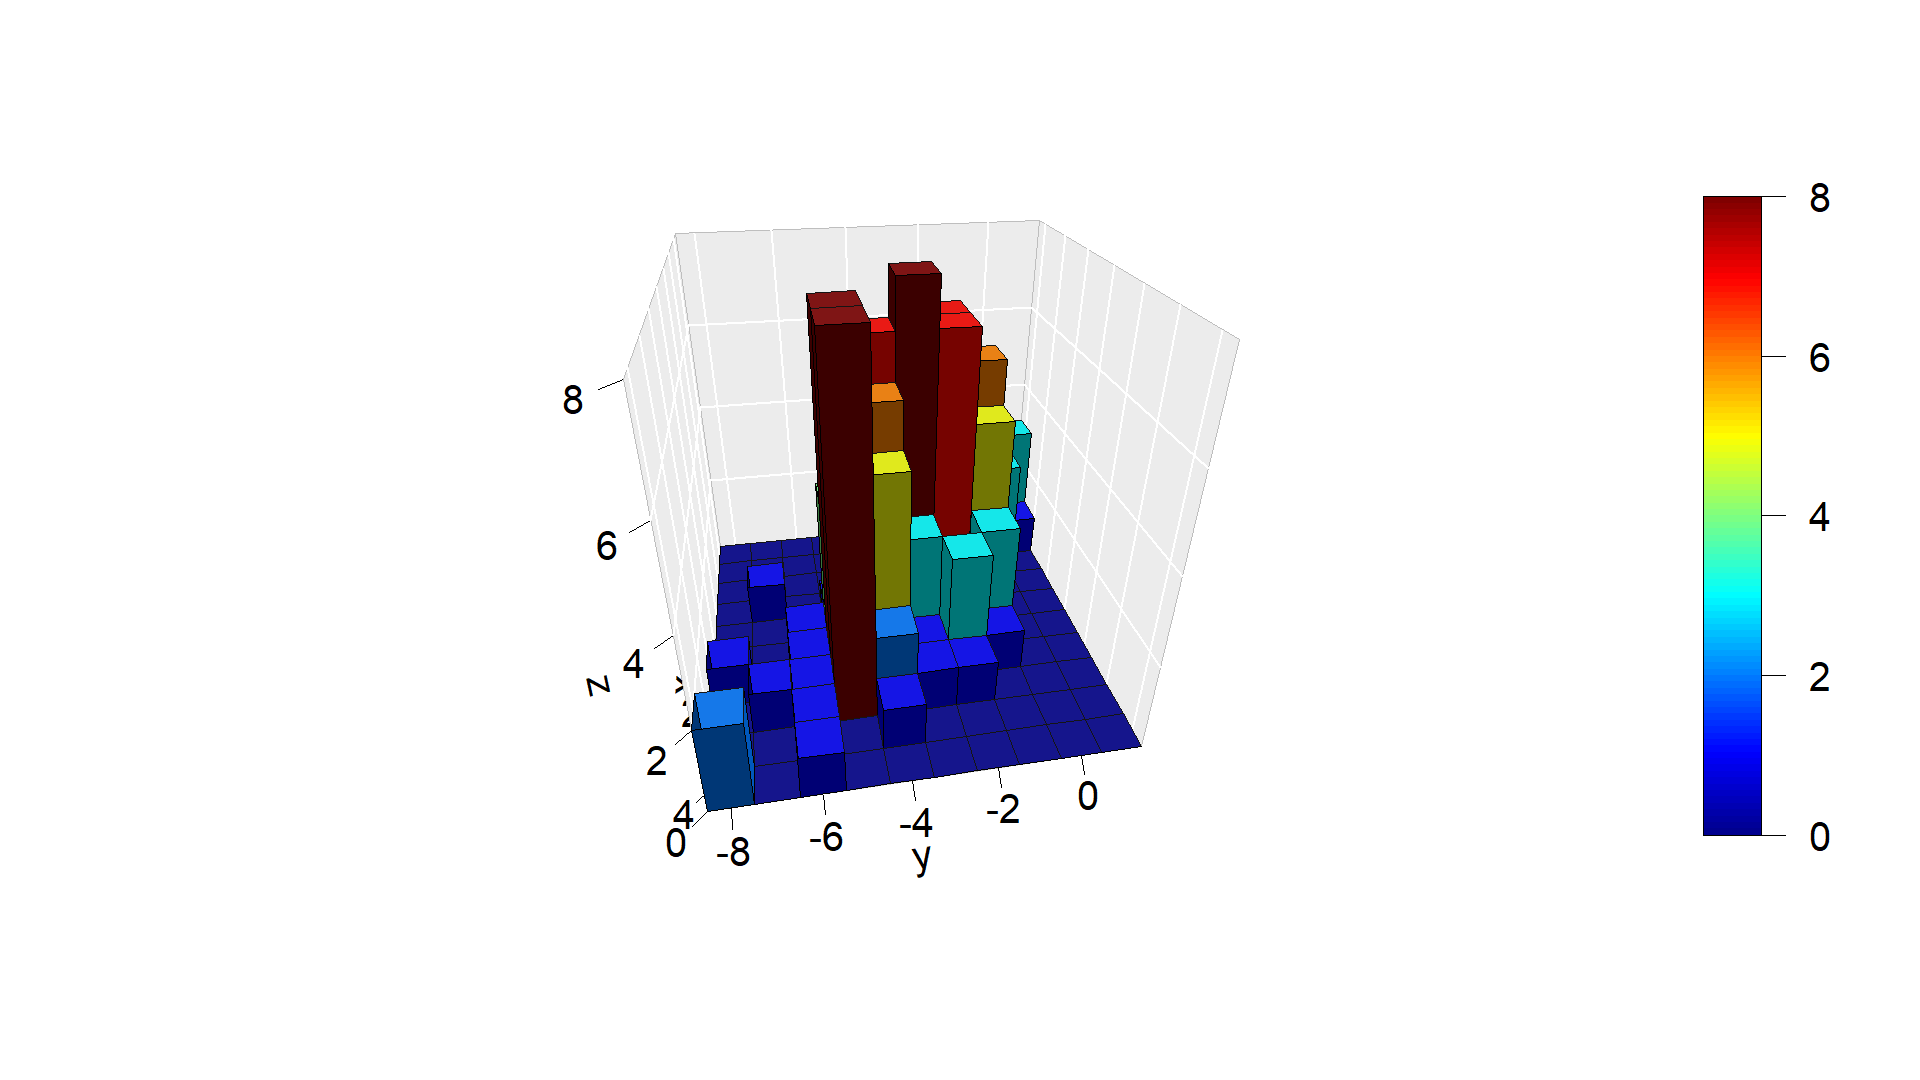
\includegraphics[width=1\linewidth]{../img/2d_2.png}} \\
	\end{minipage}
\end{figure}


\begin{figure}[H]
\begin{minipage}[h]{1\linewidth}
	\center{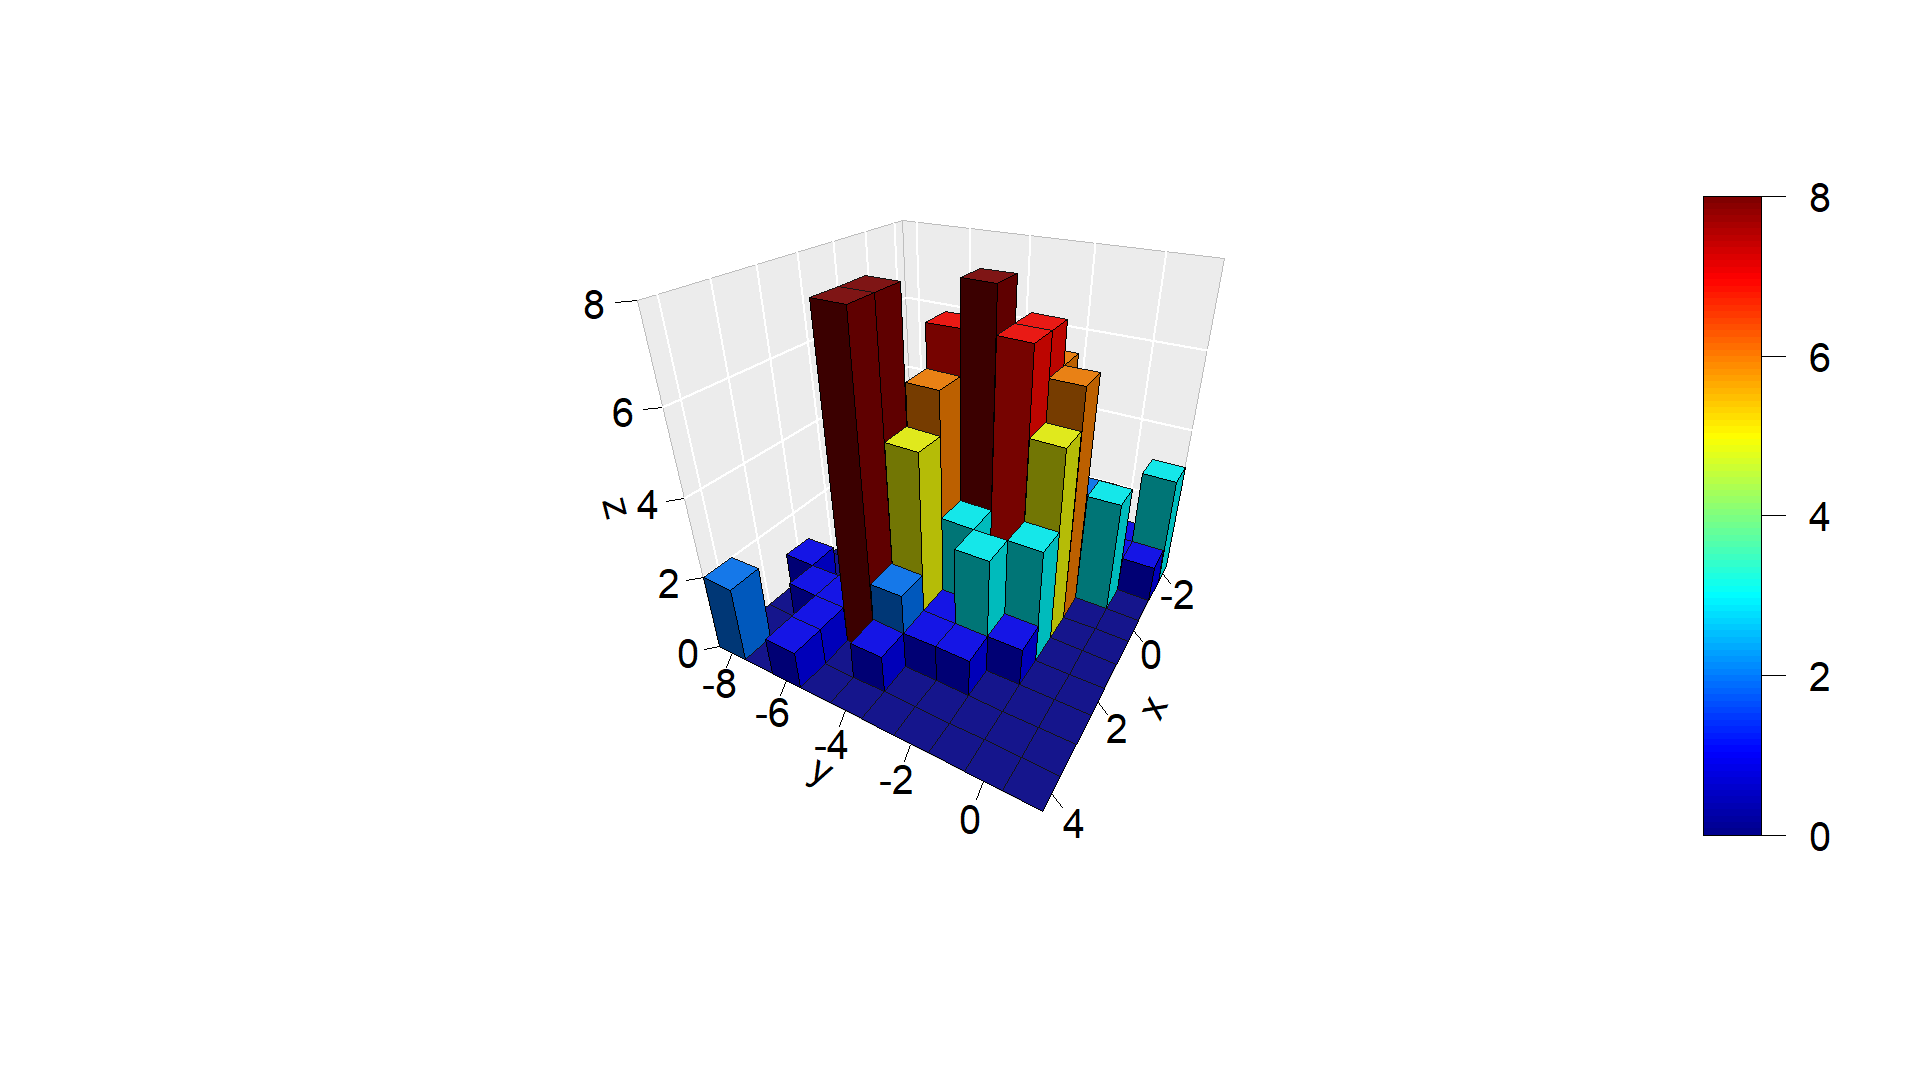
\includegraphics[width=1\linewidth]{../img/2d_3.png}} \\
\end{minipage}
\hfill
\begin{minipage}[h]{1\linewidth}
	\center{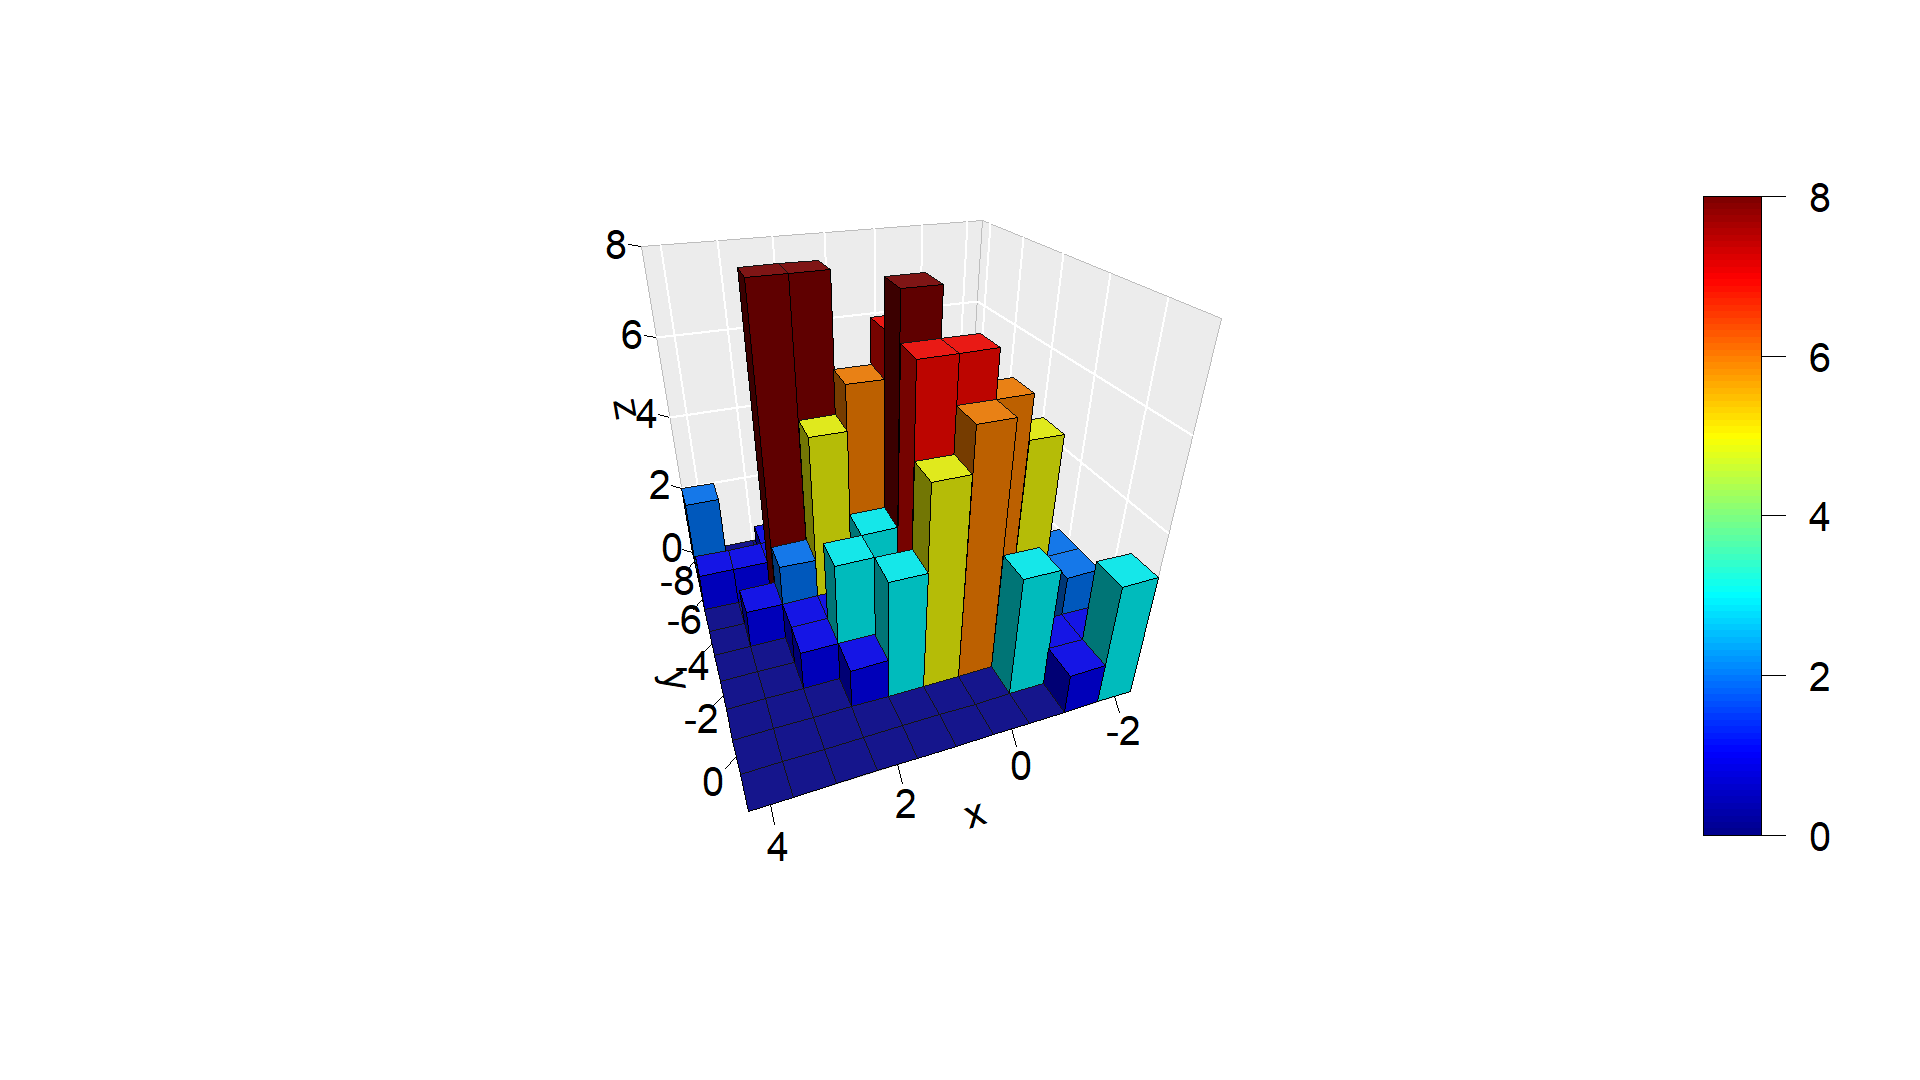
\includegraphics[width=1\linewidth]{../img/2d_4.png}} \\
\end{minipage}
\end{figure}
\begin{figure}[H]
	\begin{minipage}[h]{1\linewidth}
		\center{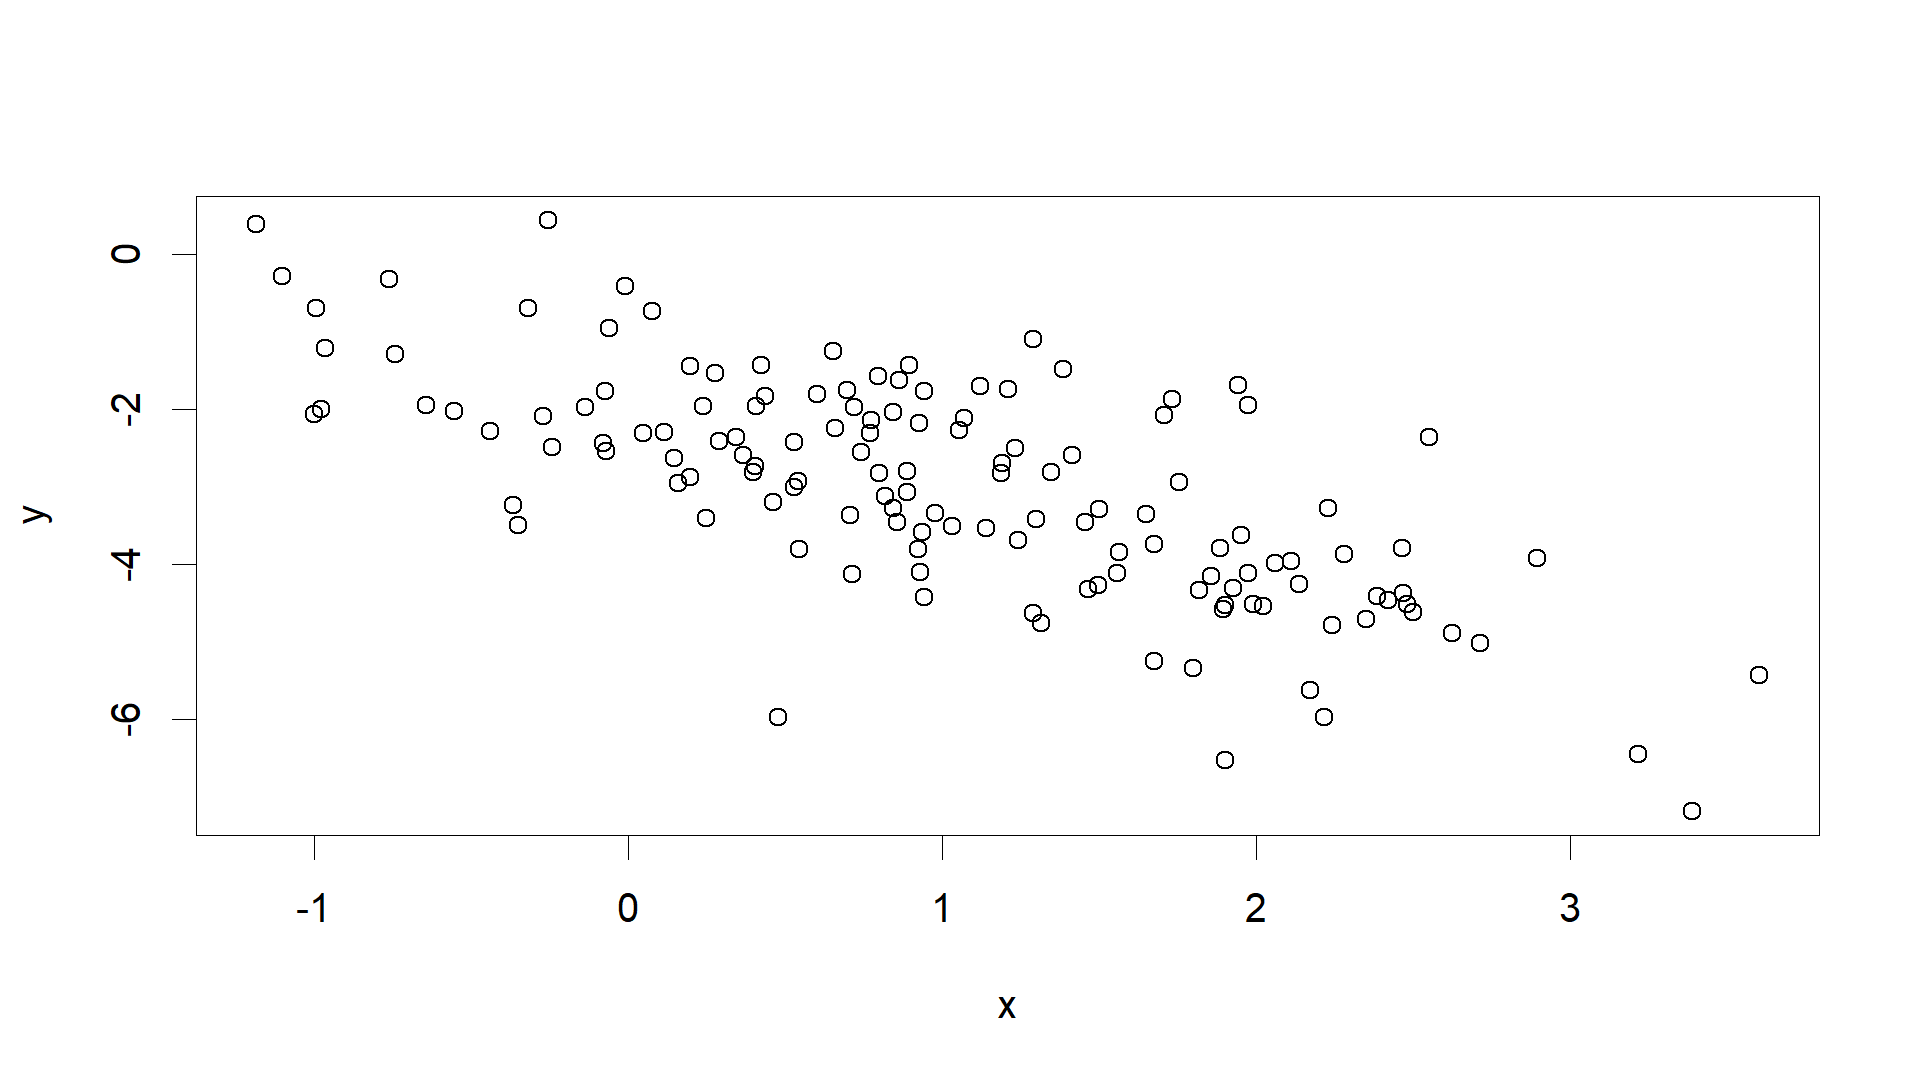
\includegraphics[width=1\linewidth]{../img/1d_without_line.png}} \\
	\end{minipage}
\end{figure}
\clearpage

\section*{Задание 2}
Найти по методу наименьших квадратов оценки коэффициентов $\hat \beta_1$ и $\hat \beta_0$ линейной регрессии $Y_k = \beta_0 + \beta_1X_k + \varepsilon_k$ И остаточной дисперсии $\hat{\delta^2}$, $D\varepsilon_k = \delta^2$. Построить совмещённые графики диаграммы рассеяния и линии регрессии.\\
\textbf{Решение.}\\
Суть МНК\footnote{В выводе используются более удобные (мне) обозначения. Далее в коде и в решении возобновляется использование Ваших обозначений}:
\begin{align}
	y_i = \beta_1 + \beta_2 \cdot x_i + \varepsilon_i\label{1}\\
	 \hat y_i = \hat \beta_1 + \hat \beta_2 \cdot x_i\label{2}
\end{align}

\begin{equation}\label{3}
	\frac{\sum\limits_{i=1}^{n}x_i}{n} = \overline{x}
\end{equation}

Из \ref{2} получаем очевидное соотношение:
\begin{equation}\label{4}
	\sum\limits_{i=1}^{n}x_i = n \cdot \overline{x} = \sum\limits_{i=1}^{n} \overline{x} \Longrightarrow \sum\limits_{i=1}^{n}(x_i - \overline{x}) = 0
\end{equation}


\begin{align}\label{5}
	RSS = \sum\limits_{i=1}^{n} (y_i - \hat y_i)^2 = \sum\limits_{i=1}^{n} (y_i-\hat b_1 - \hat \beta_2\cdot x_i)^2 = Q(\hat \beta_1,\hat \beta_2)
\end{align}

$Q(\hat \beta_1,\hat \beta_2) \longrightarrow \min$
\begin{equation}\label{6}
\begin{cases} 
	\pdv{Q}{\hat \beta_1} = \sum\limits_{i=1}^{n}2(y_i - \hat \beta_1 - \hat \beta_2\cdot x_i)(-1) = 0 \\
	\pdv{Q}{\hat \beta_2} = \sum\limits_{i=1}^{n}2(y_i - \hat \beta_1 - \hat \beta_2\cdot x_i)(-x_i) = 0 \\ 
\end{cases}
\end{equation}

(\ref{6}) $\Longrightarrow$ $(\hat \beta_1,\hat \beta_2)$\\
Заметим, что выражение в скобках в (\ref{6}) является ошибкой прогноза $\hat \varepsilon_i$. Тогда наша система (\ref{6}) перепишется в более простом виде:
\begin{equation}\label{7}
\begin{cases} 
	\sum\limits_{i=1}^{n}\hat \varepsilon_i \cdot 1 = 0 \\
	\sum\limits_{i=1}^{n}\hat \varepsilon_i \cdot x_i = 0 \\ 
\end{cases}	
\end{equation}

Для нахождения $\hat \beta_1,\hat \beta_2$ решим относительно них систему (\ref{6}):

\begin{equation}\label{8}
\begin{cases} 
\sum\limits_{i=1}^{n}y_i - \sum\limits_{i=1}^{n}\hat \beta_1 - \sum\limits_{i=1}^{n} \hat \beta_2 \cdot x_i = 0 \\
\sum\limits_{i=1}^{n}y_ix_i - \sum\limits_{i=1}^{n}\hat\beta_1 x_i - \sum\limits_{i=1}^{n}\hat\beta_2x_i^2 = 0 \\ 
\end{cases}	
\end{equation}


\begin{equation}\label{9}
\begin{cases} 
	\sum\limits_{i=1}^{n}y_i - n\beta_1 - \hat \beta_2 \sum\limits_{i=1}^{n}  x_i = 0 \\
	\sum\limits_{i=1}^{n}y_ix_i - \hat\beta_1\sum\limits_{i=1}^{n} x_i - \hat\beta_2\sum\limits_{i=1}^{n}x_i^2 = 0 \\ 
\end{cases}	
\end{equation}

Из первого уравнения (\ref{9}) при делении на n следует:
\begin{equation}\label{10}
	\overline{y} - \hat \beta_1 - \hat \beta_2 \overline{x} = 0
\end{equation}

Или

\begin{equation}\label{11}
\overline{y} = \hat \beta_1 + \hat \beta_2 \overline{x}
\end{equation}

Выразим $\beta_1$ из (\ref{11}) и подставим во второе уравнение (\ref{9}):

\begin{equation}\label{12}
	\hat\beta_1 = \overline{y} - \hat \beta_2 \cdot \overline{x}
\end{equation}

\begin{equation}\label{13}
	\sum\limits_{i=1}^{n} y_ix_i - (\overline{y} - \hat\beta_2\cdot\overline{x})\sum\limits_{i=1}^{n}x_i - \hat\beta_2\sum\limits_{i=1}^{n}x_i^2 = 0
\end{equation}

\begin{equation}\label{14}
	\sum\limits_{i=1}^{n} y_ix_i - \overline{y}\sum\limits_{i=1}^{n}x_i + \hat\beta_2\cdot\overline{x}\sum\limits_{i=1}^{n}x_i - \hat\beta_2\sum\limits_{i=1}^{n}x_i^2 = 0
\end{equation}


\begin{equation}\label{15}
	\hat\beta_2 (\overline{x}\sum\limits_{i=1}^{n}x_i - \sum\limits_{i=1}^{n}x_i^2) = \overline{y}\sum\limits_{i=1}^{n}x_i - \sum\limits_{i=1}^{n}y_ix_i
\end{equation}

\begin{equation}\label{16}
	\hat\beta_2 = \frac{\overline{y}\sum\limits_{i=1}^{n}x_i - \sum\limits_{i=1}^{n}y_ix_i}{\overline{x}\sum\limits_{i=1}^{n}x_i - \sum\limits_{i=1}^{n}x_i^2}
\end{equation}

Уже получили правильный ответ, но приведём решение к более красивому виду:

\begin{equation}\label{17}
	\hat\beta_2 = \frac{\sum\limits_{i=1}^{n}y_ix_i - \sum\limits_{i=1}^{n}\overline{y}x_i}{\sum\limits_{i=1}^{n}x_i^2 - \sum\limits_{i=1}^{n}\overline{x}x_i} = \frac{\sum\limits_{i=1}^{n}(y_i - \overline{y})x_i}{\sum\limits_{i=1}^{n}(x_i-\overline{x})x_i}
\end{equation}

Тут уже лучше видно, что числитель и знаменатель похожи. Но сделаем ещё одно преобразование, которое из правильного ответа сделает правильный ответ.

Вспомним про (\ref{4}). Из него следует интересный факт:

\begin{equation}\label{18}
	\sum\limits_{i=1}^{n}(x_i - \overline{x}) = 0 \Longrightarrow \overline{x}\sum\limits_{i=1}^{n}(x_i-\overline{x}) = 0 \Longrightarrow \sum\limits_{i=1}^{n}\overline{x}(x_i-\overline{x}) = 0 
\end{equation}

Тогда вычтем нули из числителя и знаменателя в (\ref{17}):

\begin{equation}\label{19}
	\hat\beta_2 = \frac{\sum\limits_{i=1}^{n}(y_i - \overline{y})x_i - \sum\limits_{i=1}^{n}\overline{x}(y_i-\overline{y})}{\sum\limits_{i=1}^{n}(x_i-\overline{x})x_i - \sum\limits_{i=1}^{n}\overline{x}(x_i-\overline{x})}
\end{equation}

Внесём всё под один знак суммы:

\begin{equation}\label{20}
	\hat\beta_2 = \frac{\sum\limits_{i=1}^{n}(y_i-\overline{y})(x_i-\overline{x})}{\sum\limits_{i=1}^{n}(x_i-\overline{x})^2}
\end{equation}


Эта форма записи хороша тем, что везде фигурируют отклонения наблюдений от среднего значения.


Таким образом получили выражения для расчёта $\hat \beta_1,\hat \beta_2$:

\begin{equation}\label{21}
	\begin{cases} 
	 \hat\beta_2 = \frac{\sum\limits_{i=1}^{n}(y_i-\overline{y})(x_i-\overline{x})}{\sum\limits_{i=1}^{n}(x_i-\overline{x})^2}\\
	 \hat\beta_1 = \overline{y} - \hat\beta_2\overline{x}\\ 
	\end{cases}	
\end{equation}

Получаем:
\begin{minted}{R}
> beta_1 <- (sum((df[,2] - meany)*(df[,1] - meanx)))/
+   (sum((df[,1] - meanx)^2))
> beta_0  <- meany - beta_1 * meanx
> beta_1
[1] -1.006984
> beta_0
[1] -1.997074
\end{minted}

Или
\begin{minted}{R}
> lm1 <- lm(df[,2] ~ df[,1])
> summary(lm1)

Call:
lm(formula = df[, 2] ~ df[, 1])

Residuals:
Min      1Q  Median      3Q     Max 
-3.4976 -0.5606 -0.1048  0.7340  2.2569 

Coefficients:
Estimate Std. Error t value Pr(>|t|)    
(Intercept) -1.99707    0.11926  -16.75   <2e-16 ***
df[, 1]     -1.00698    0.08379  -12.02   <2e-16 ***
---
Signif. codes:  0 ‘***’ 0.001 ‘**’ 0.01 ‘*’ 0.05 ‘.’ 0.1 ‘ ’ 1

Residual standard error: 0.9912 on 138 degrees of freedom
Multiple R-squared:  0.5114,	Adjusted R-squared:  0.5078 
F-statistic: 144.4 on 1 and 138 DF,  p-value: < 2.2e-16
\end{minted}

Видим, что результаты совпадают.

Можем записать полученное уравнение линейной регрессии:

\begin{equation*}
	Y = -1.00698 -1.99707\cdot X
\end{equation*}


Остаточная дисперсия равна
\begin{equation*}
	\hat{\delta}^{2}=\frac{1}{n-2} \sum_{k=1}^{n}\left(Y_{k}-\hat{\beta}_{0}-\hat{\beta}_{1} X_{k}\right)^{2}
\end{equation*}

\begin{minted}{R}
> sigma_ost <- (sum((df[,2] - beta_1 * 
+                      df[,1] - beta_0)^2))/(n-2)
> sigma_ost
[1] 0.9824018
\end{minted}


Построим совмещённые графики диаграммы рассеяния и линии регрессии:

\begin{minted}{R}
> plot(df)
> abline(lm1)
\end{minted}


\begin{figure}[H]
	\begin{minipage}[h]{1\linewidth}
		\center{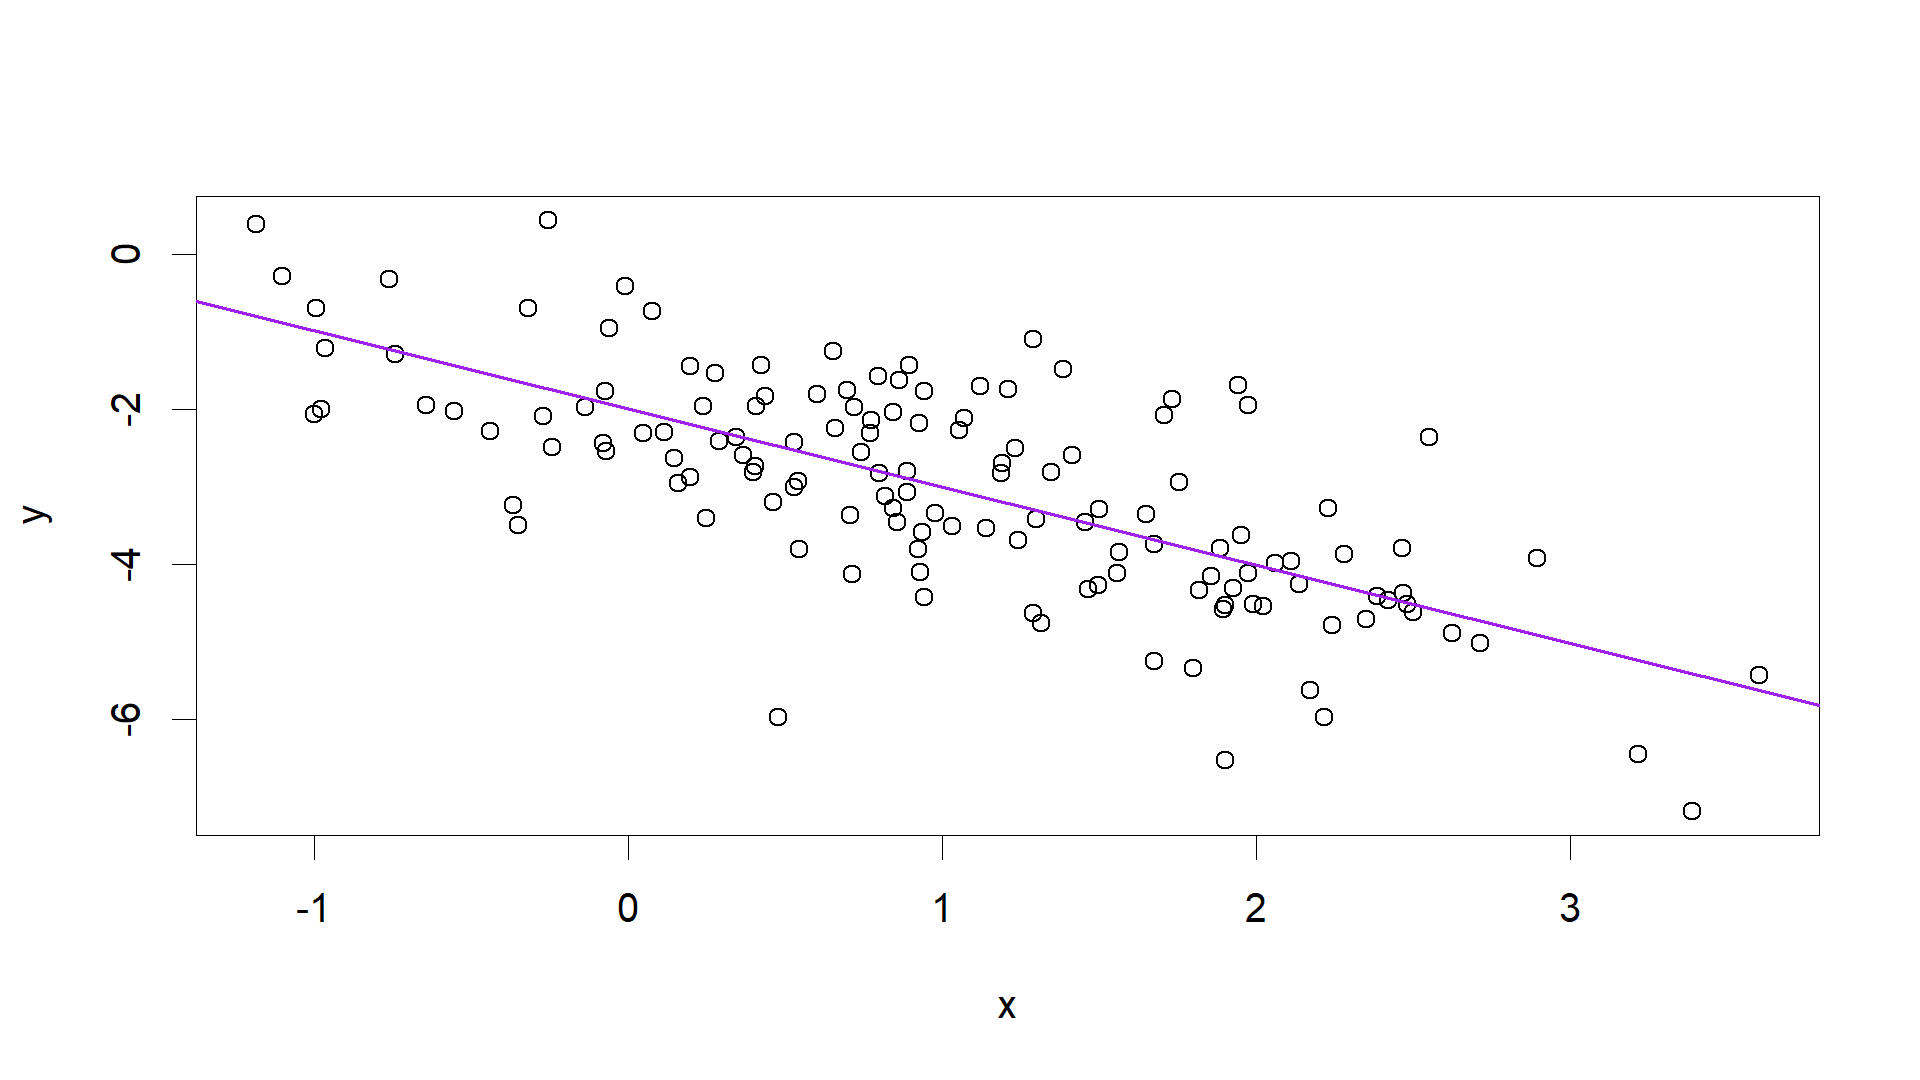
\includegraphics[width=1\linewidth]{../img/1d_line.png}}  \\
	\end{minipage}
\end{figure}

\clearpage 
\section*{Задание 3}
Найти доверительные интервалы с доверительной вероятностью $1-\alpha = 0.95$
\subsection*{1. Доверительные интервал для коэффициента корреляции компонент $r$}

Рассмотрим следующие статистики:
\begin{align*}
	\begin{aligned} \mu_{20}=& \frac{1}{n} \sum_{k=1}^{n}\left(X_{k}-\bar{X}\right)^{2}\\ \mu_{02}=& \frac{1}{n} \sum_{k=1}^{n}\left(Y_{k}-\bar{Y}\right)^{2}\\ \mu_{11}=& \frac{1}{n} \sum_{k=1}^{n}\left(X_{k}-\bar{X}\right)\left(Y_{k}-\bar{Y}\right) \end{aligned}
\end{align*}

\begin{minted}{R}
> mu20 <- 1/n * sum((df[,1] - meanx)^2)
> mu20
[1] 0.9994035
> mu02 <- 1/n * sum((df[,2] - meany)^2)
> mu02
[1] 1.98178
> mu11 <- 1/n * sum((df[,1] - meanx)*(df[,2] - meany))
> mu11
[1] -1.006384
\end{minted}

Тогда выборочный коэффициент корреляции равен:
\begin{equation*}
	r_\textup{В} = \frac{\mu_{11}}{\sqrt{\mu_{20}\mu_{02}}}
\end{equation*}

\begin{minted}{R}
> rv <- mu11/sqrt(mu20*mu02)
> rv
[1] -0.7150978
\end{minted}

Рассмотрим статистику $z = \frac{1}{2} \ln{\frac{1+r_\textup{В}}{1-r_\textup{В}}} = \atanh{r_\textup{В}}$, которая при $n \geq 10$ приближённо распределена $\sim N(a_z, \frac{1}{\sqrt{n-3}})$, где $a_z = \atanh(r) + \frac{r}{(2n-1)}$.

Следовательно, $(z-a_z)\sqrt{n-3} \sim N(0,1)$.

Доверительный интервал для коэффициента корреляции компонент $r$:

\begin{align*}
&1-\alpha = P\Big(-u_{1-\frac{\alpha}{2}}<(z-a_z)\sqrt{n-3} <u_{1-\frac{\alpha}{2}}
\Big)=P\Big(z-\frac{u_{1-\frac{\alpha}{2}}}{\sqrt{n-3}}<a_z <z+\frac{u_{1-\frac{\alpha}{2}}}{{\sqrt{n-3}}}
\Big)= \\
&= P\Big(\atanh \ r_{\text{в}}-\frac{u_{1-\frac{\alpha}{2}}}{\sqrt{n-3}}<\atanh \ r +\frac{r}{2(n-1)} <\atanh \ r_{\text{в}}+\frac{u_{1-\frac{\alpha}{2}}}{{\sqrt{n-3}}}
\Big)
\end{align*}
Итого:
\begin{equation*}
\resizebox{\textwidth}{!}
{%
	${P\Big(\tanh(\atanh \ r_{\text{в}}-\frac{r_{\text{в}}}{2(n-1)}-\frac{u_{1-\frac{\alpha}{2}}}{\sqrt{n-3}})< r  < \tanh(\atanh \ r_{\text{в}}-\frac{r_{\text{в}}}{2(n-1)}+\frac{u_{1-\frac{\alpha}{2}}}{{\sqrt{n-3}}})\Big)}$%
}
\end{equation*}

Получаем:

\begin{minted}{R}
> CIr_lower_bound <- tanh(atanh(rv) - rv/(2*(n-1)) 
+                         - qnorm(1-alpha/2)/sqrt(n-3))
> CIr_lower_bound
[1] -0.7865877
> CIr_upper_bound <- tanh(atanh(rv) - rv/(2*(n-1)) 
+                         + qnorm(1-alpha/2)/sqrt(n-3))
> CIr_upper_bound
[1] -0.6215435
\end{minted}

Получаем доверительный интервал:
\begin{equation*}
	-0.7865877 \leq r \leq -0.6215435
\end{equation*}

Истинное значение коэффициента корреляции
\begin{equation*}
	r = \frac{\sigma_{12}}{\sqrt{\sigma_{11}\sigma_{22}}} = -0.7071068
\end{equation*}
попадает в полученный интервал.

\subsection*{2. Доверительный интервал для коэффициентов регрессии $\beta_0$ и $\beta_1$}

Запишем матрицу базисных функций:

\begin{equation*}
	F=
	\begin{pmatrix}
		1& X_1 \\
		\ldots &\ldots\\
		1 & X_n
	\end{pmatrix},
	\qquad
	F^T=
	\begin{pmatrix}
		1& \ldots&1 \\
		X_1 &\ldots&X_n\\
	\end{pmatrix}
\end{equation*}

\begin{equation*}
	F^TF=\begin{pmatrix}
	1& ...&1 \\
	X_1 &...&X_n\\
	
	
	
	\end{pmatrix}\begin{pmatrix}
	1& X_1 \\
	... &...\\
	
	1 & X_n
	
	
	\end{pmatrix}=\begin{pmatrix}
	n& \sum\limits_{k=1}^nX_k \\
	\sum\limits_{k=1}^nX_k & \sum\limits_{k=1}^nX_k^2
	
	
	
	\end{pmatrix}=
	\begin{pmatrix}
	140& 141.8275 \\
	141.8275 & 283.5953
	
	
	
	\end{pmatrix}
\end{equation*}

\begin{equation*}
	(F^TF)^{-1}=\frac {1}{n\sum\limits_{k=1}^nX_k^2-\Big(\sum\limits_{k=1}^nX_k^2\Big)^2}\begin{pmatrix}
	\sum\limits_{k=1}^nX_k^2& -\sum\limits_{k=1}^nX_k \\
	-\sum\limits_{k=1}^nX_k & n
	
	
	
	\end{pmatrix}=\begin{pmatrix}
	0.014477&  -0.007240 \\
	-0.007240& 0.007147
	
	
	
	\end{pmatrix}
\end{equation*}

$\hat \beta_i \sim N(\beta_i, \hat\delta \sqrt{\tau_{ii}})$, где $\tau_{ii}$ -- элемент матрицы $(F^TF)^{-1}$.


В общем случаем доверительный интервал для коэффициента регрессии $\beta_i$ В случае $\varepsilon_k \sim N(0,\delta)$ при неизвестном $\delta$:

\begin{equation*}
	\hat{\beta}_{i}-t_{1-\frac{\alpha}{2}}(n-m) \hat{\delta} \sqrt{\tau_{i i}}<\beta_{i}<\hat{\beta}_{i}+t_{1-\frac{\alpha}{2}}(n-m) \hat{\delta} \sqrt{\tau_{i i}}
\end{equation*}


Доверительный интервал для коэффициента регрессии $\beta_0$:


\begin{equation*}
	\hat{\beta}_{0}-t_{1-\frac{\alpha}{2}}(n-m) \hat{\delta} \sqrt{\tau_{11}}<\beta_{0}<\hat{\beta}_{0}+t_{1-\frac{\alpha}{2}}(n-m) \hat{\delta} \sqrt{\tau_{11}}
\end{equation*}

\begin{minted}{R}
> M <- matrix(c(n, sum(df[,1]), 
+               sum(df[,1]),sum((df[,1])^2)), 
+             ncol = 2, byrow = T)
> M_obr <- solve(M)
> 
> 
> 
> CIbeta0_lower_bound <- beta_0 - 
+   qt(1-alpha/2, n-2) * sqrt(sigma_ost) * sqrt(M_obr[1,1])
> CIbeta0_lower_bound
[1] -2.232888
> CIbeta0_upper_bound <- beta_0 + 
+   qt(1-alpha/2, n-2) * sqrt(sigma_ost) * sqrt(M_obr[1,1])
> CIbeta0_upper_bound
[1] -1.76126
\end{minted}

Получаем доверительный интервал для $\beta_0$:
\begin{equation*}
	-2.232888 \leq \beta_0 \leq -1.76126
\end{equation*}

Доверительный интервал для коэффициента регрессии $\beta_1$:
\begin{equation}
	\hat{\beta}_{1}-t_{1-\frac{\alpha}{2}}(n-m) \hat{\delta} \sqrt{\tau_{11}}<\beta_{1}<\hat{\beta}_{1}+t_{1-\frac{\alpha}{2}}(n-m) \hat{\delta} \sqrt{\tau_{11}}
\end{equation}

\begin{minted}{R}
> CIbeta1_lower_bound <-  beta_1 - 
+   (qt(1-alpha/2, n-2) * sqrt(sigma_ost)) * sqrt(M_obr[2,2])
> CIbeta1_lower_bound
[1] -1.17267
> CIbeta1_upper_bound <-  beta_1 + 
+   (qt(1-alpha/2, n-2) * sqrt(sigma_ost)) * sqrt(M_obr[2,2])
> CIbeta1_upper_bound
[1] -0.8412993
\end{minted}

Получаем доверительный интервал для $\beta_1$:

\begin{equation*}
-1.17267 \leq \beta_1 \leq -0.8412993
\end{equation*}

Или
\begin{minted}{R}
> confint(lm1)
	      2.5 %     97.5 %
(Intercept) -2.232888 -1.7612602
df[, 1]     -1.172670 -0.8412993
\end{minted}

\subsection*{3. Доверительный интервал для дисперсии $\delta^2$}

Доверительный интервал для $\delta^2$ в случае $\varepsilon_k \sim N(0,\delta)$ при неизвестном $\delta$:

\begin{equation*}
	\frac{\hat{\delta}^{2}(n-2)}{\delta^{2}} \sim \chi^{2}(n-2)	
\end{equation*}

\begin{equation*}
	\chi_{\frac{\alpha}{2}}^{2}(n-2)<\frac{\hat{\delta}^{2}(n-2)}{\delta^{2}}<\chi_{1-\frac{\alpha}{2}}^{2}(n-2)
\end{equation*}


Следовательно:
\begin{equation*}
\frac{\hat{\delta}^{2}(n-2)}{\chi_{1-\frac{\alpha}{2}}^{2}(n-2)}<\delta^{2}<\frac{\hat{\delta}^{2}(n-2)}{\chi_{\frac{\alpha}{2}}^{2}(n-2)}
\end{equation*}

\begin{minted}{R}
> CIdelta_ost_upper_boud<- (n-2)*delta_ost / 
+   (qchisq(alpha/2, n-2))
> CIdelta_ost_upper_boud
[1] 1.26263
> CIdelta_ost_lower_boud <- (n-2)*delta_ost / 
+   (qchisq(1-alpha/2, n-2))
> CIdelta_ost_lower_boud
[1] 0.7863207
\end{minted}

Получаем доверительный интервал для $\delta^2$:
\begin{equation*}
	0.7863207 \leq \delta^2 \leq 1.26263
\end{equation*}








\end{document}